% Drawing 146/03-5 -- folder 146, batch 03, archive page 59 (PDF page 60).
% Transcription: à gauche, « III » : une sphère portant deux cercles parallèles reliés par deux montants verticaux, le cercle du haut « cercle marqué », deux sommets cerclés sur le cercle du bas et deux au pôle ; « $\mathbb{Z}/2$ » ; légende « $9 = 3 + 3 + 1 + 2$ sommets, 6 faces, 1 cercle marqué » ; « $60 = 10 \times 3 \times 2$ poss.\ pour $K$ » ; « (triangle + sommet marqué + \ill{}) » avec sous les termes 10, 3, 2. Au centre, un schéma en « $\vee\!\!\perp\!\vee$ » à deux branches. À droite : « $D_0$ », « III » : une sphère à équateur portant cinq sommets cerclés, marquée « $D_5$ » ; légende « \struck{12 façons} 5 sommets, 2 faces, 12 possibilités qui \ill{} orientation de $K$ » ; « IV », « $D_2$ » : une sphère méridienne en fuseaux avec trois sommets cerclés ; légende « \struck{\ill{}} sommets, 6 faces, 20 possibilités (cf \ill{}, car il faut choisir une orientation de la sphère) $\sim$ orientation de $K$ » ; un croquis raturé « $\mathfrak{S}_3$ ».
% Kind: cell decompositions of the sphere (page of cases). Method 3 (encoded, rendered from the data). Status: partial.
% Notes: III (left): two parallel circles joined by two posts, the top one « cercle marqué », a pole axis, ringed vertices at the pole, at the centre and on the bottom circle -- redrawn; his count « 9 = 3+3+1+2 sommets, 6 faces » is NOT encoded, because the figure alone does not fix where the 3+3+1+2 vertices sit. D0 / D5 (right, top): equator with five ringed vertices, encoded (V=5, F=2, as he writes). IV / D2: sphere in lunes with three ringed vertices, redrawn only (meridians approximate; his vertex count is struck). The struck S3 sketch and the small faint circle top right drawn grey. The loose dots and the forked segment along the bottom edge of the bbox are left out (their reading belongs to the text below). Legends abridged to their counts.
% Coordinates: 1 unit = 1 mm = 1/100 of the crop width (bbox in page fractions: [0.08, 0.08, 0.95, 0.48]).
% Redrawn by Claude (claude-opus-5-5), issue #73 pilot, 2026-11-07; not checked by a human; not compiled (no TeX in the session).
% Rights: reproduces part of the work -- behind RENDER_TRANSCRIPTS, never published by itself.
\documentclass[tikz,border=3pt]{standalone}
\usepackage{amsmath,amssymb}
\usetikzlibrary{patterns,arrows.meta}
\tikzset{pencil/.style={black!45}, struck/.style={black!35}, mark/.style={circle,draw,inner sep=1.3pt}, pt/.style={circle,fill,inner sep=0.9pt}, opt/.style={circle,draw,fill=white,inner sep=1.1pt}}
\begin{document}
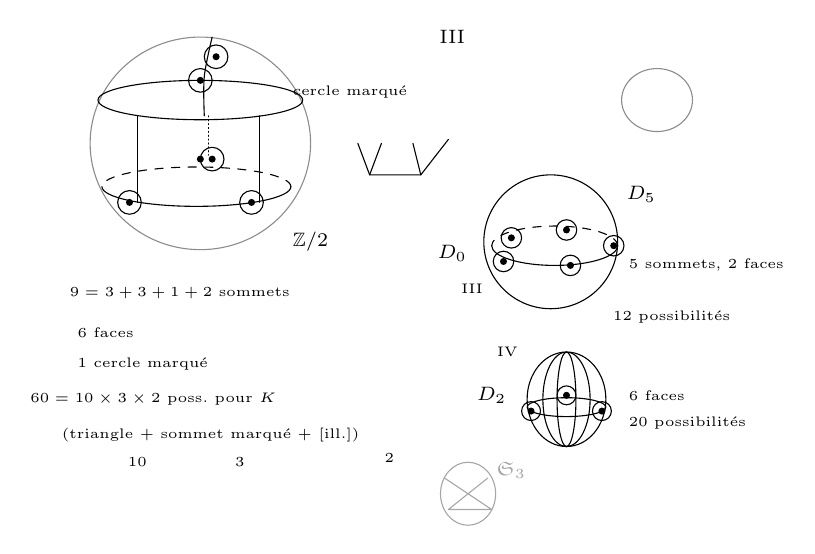
\begin{tikzpicture}[x=1mm,y=1mm,line cap=round,line join=round,font=\scriptsize]
\draw[pencil] (27,-16.5) ellipse[x radius=14, y radius=13.5];
\draw (27,-11) ellipse[x radius=13, y radius=2.5];
\draw[dashed] (38.5,-22) arc[start angle=0, end angle=180, x radius=12, y radius=2.5];
\draw (14.5,-22) arc[start angle=180, end angle=360, x radius=12, y radius=2.5];
\draw (19,-13) -- (19,-24);
\draw (34.5,-13) -- (34.5,-24);
\draw plot[smooth, tension=0.55] coordinates {(27.5,-13) (27.5,-8) (28.5,-3)};
\draw[densely dotted] (28,-13) -- (28,-18);
\draw (29,-5.5) circle[radius=1.5];
\draw (27,-8.5) circle[radius=1.5];
\draw (28.5,-18.5) circle[radius=1.5];
\draw (18,-24) circle[radius=1.5];
\draw (33.5,-24) circle[radius=1.5];
\node[pt] at (29,-5.5) {};
\node[pt] at (27,-8.5) {};
\node[pt] at (28.5,-18.5) {};
\node[pt] at (18,-24) {};
\node[pt] at (33.5,-24) {};
\node[pt] at (27,-18.5) {};
\node[inner sep=1pt] at (46,-10) {\tiny cercle marqué};
\node[inner sep=1pt] at (41,-29) {\scriptsize $\mathbb{Z}/2$};
\draw (47,-16.5) -- (48.5,-20.5) -- (55,-20.5) -- (58.5,-16);
\draw (50,-16.5) -- (48.5,-20.5);
\draw (54,-16.5) -- (55,-20.5);
\node[inner sep=1pt,anchor=west] at (10,-35.5) {\tiny $9=3+3+1+2$ sommets};
\node[inner sep=1pt,anchor=west] at (11,-40.5) {\tiny 6 faces};
\node[inner sep=1pt,anchor=west] at (11,-44.5) {\tiny 1 cercle marqué};
\node[inner sep=1pt,anchor=west] at (5,-49) {\tiny $60=10\times3\times2$ poss.\ pour $K$};
\node[inner sep=1pt,anchor=west] at (9,-53.5) {\tiny (triangle + sommet marqué + [ill.])};
\node[inner sep=1pt] at (19,-57) {\tiny 10};
\node[inner sep=1pt] at (32,-57) {\tiny 3};
\node[inner sep=1pt] at (51,-56.5) {\tiny 2};
\node[inner sep=1pt] at (59,-3) {\scriptsize III};
\draw (71.5,-29) circle[radius=8.5];
\draw[dashed] (80,-29.5) arc[start angle=0, end angle=180, x radius=8, y radius=2.5];
\draw (64,-29.5) arc[start angle=180, end angle=360, x radius=8, y radius=2.5];
\draw (66.5,-28.5) circle[radius=1.3];
\draw (73.5,-27.5) circle[radius=1.3];
\draw (79.5,-29.5) circle[radius=1.3];
\draw (65.5,-31.5) circle[radius=1.3];
\draw (74,-32) circle[radius=1.3];
\node[pt] at (66.5,-28.5) {};
\node[pt] at (73.5,-27.5) {};
\node[pt] at (79.5,-29.5) {};
\node[pt] at (65.5,-31.5) {};
\node[pt] at (74,-32) {};
\node[inner sep=1pt] at (59,-30.5) {\scriptsize $D_0$};
\node[inner sep=1pt] at (83,-23) {\scriptsize $D_5$};
\node[inner sep=1pt] at (61.5,-35) {\tiny III};
\node[inner sep=1pt,anchor=west] at (81,-32) {\tiny 5 sommets, 2 faces};
\node[inner sep=1pt,anchor=west] at (79,-38.5) {\tiny 12 possibilités};
\draw (73.5,-49) ellipse[x radius=5, y radius=6];
\draw (73.5,-49) ellipse[x radius=3, y radius=6];
\draw (73.5,-49) ellipse[x radius=1.2, y radius=6];
\draw (73.5,-50) ellipse[x radius=5, y radius=1.2];
\draw (73.5,-48.5) circle[radius=1.2];
\draw (69,-50.5) circle[radius=1.2];
\draw (78,-50.5) circle[radius=1.2];
\node[pt] at (73.5,-48.5) {};
\node[pt] at (69,-50.5) {};
\node[pt] at (78,-50.5) {};
\node[inner sep=1pt] at (66,-43) {\tiny IV};
\node[inner sep=1pt] at (64,-48.5) {\scriptsize $D_2$};
\node[inner sep=1pt,anchor=west] at (81,-48.5) {\tiny 6 faces};
\node[inner sep=1pt,anchor=west] at (81,-52) {\tiny 20 possibilités};
\draw[struck] (61,-61) ellipse[x radius=3.5, y radius=4];
\draw[struck] (58,-59) -- (64,-63) -- (58.5,-63) -- (63.5,-59);
\node[inner sep=1pt,struck] at (66.5,-58) {\scriptsize $\mathfrak{S}_3$};
\draw[pencil] (85,-11) ellipse[x radius=4.5, y radius=4];
\end{tikzpicture}
\end{document}
